\chapter{引言}

\section{CMB的小尺度变化}

地球的核幔边界(CMB)在地球内部的动力学演化过程中具有非常关键的作用,由于它和地幔、地核的对流有
着紧密的联系,对其性质的了解有助于我们认识地球的演化. 许多地震学的研究揭示了这个界面存在复杂的性质并
伴有强烈的区域性变化. 

在这些可能存在的复杂结构中,超低速带(ULVZ)常常受到关注. 它的典型特征是具有低的P和S波波速,并较周围结
构有更高的密度,前人的研究发现这种结构常常存在于大剪切波低速省的附近~\citep{Garnero2008}. ULVZ通
常被认为尺度很小(约数百千米),因此也较难用层析成像等地震学手段探测到. 之前的研究常基于异常大的PKP前驱波~\citep{vidale1998evidence,Thomas2009}或者异常的SKP${}_{diff}$S走时延迟~\citep{Thorne2004a,Garnero1995}来推断ULVZ的存在,在一些研究中,短周期的PcP和ScP被
用来提高对CMB结构探测的分辨率~\citep{Castle2000,Rost2004a}. ULVZ的存在可能造成PcP的复杂特性,
当低速带与其上部地幔有较大速度差的情况下,PcP主震相前将出现由ULVZ顶部反射的前驱波,其后可能出现P到S
波的转换震相,并且由于反射系数的减小,PcP的振幅也会显著降低~\citep{Gassner2015}. 目前多数研究认为这种低速结构的形成可能是源于CMB上部物质的部分熔融,比如含水的洋中脊玄武岩(MORB)下沉到地幔底部,降低了周围物质的熔点而产生熔融,而且这些MORB受到地幔对流的影响更易于集中在化学性质差异明显的边界比如LLSVPs的周围~\citep{Xu2009a}. 除此之外还有一些其他的机制用来解释其成因,有实验模拟研究认为这种低速结构来源于地幔于外核物质的化学反应~\citep{Hirose2005a},或者CMB底部的物质沉积~\citep{Buffett2000a}. \citet{He2006a,He2012a}通过ScS-S、ScS2-SS走时残差和波形模拟尝试确定了太平洋低速异常的边界,并认为太平洋边界底部的ULVZ从异常内延伸到周围的高速区,并且这种扩张在小尺度内存在强烈变化,这暗示了太平洋异常低速异常可能存在变化的物质组成以及同周围地幔物质复杂的接触关系. 

CMB另一个重要的特征是它的界面起伏,根据之前的研究结果,其横向尺度可能从数百至数千千米;深度变化从几
百米至数百千米~\citep{Earle1997,Sze200327}. CMB的界面起伏会强烈影响PcP的观测,一个局部上凸的界面会造成波场
能量的发散,因此减小PcP的振幅,而一个局部下陷的CMB界面会产生相反的效果,即造成能量的汇聚,从而增大PcP的振幅~\citep{Kampfmann1989a,Neuberg1991}. \citet{Rost2004a}利用Yellow Knife台阵观测
到异常大的PcP振幅,并结合P作为参考震相进行分析,认为在阿拉斯加的Kenai半岛下方的CMB上存在局部的下凹. 最近,\cite{Wu2014a}利用表示定理模拟了不同横向尺度和深度变化参数组合的CMB起伏下的PcP
波形,结合之前在Kenai半岛下方CMB反射的PcP数据,检验了CMB界面起伏对PcP的影响. 其结果显示,一个下陷6千米,横
向宽度6{\textdegree}的界面起伏会造成PcP振幅放大4.5倍. 但是,在P波衰减和PcP振幅增大之间仍然存在一
个折衷效应,因为之前的研究通常使用P作为参考震相,而在上地幔中,直达P波和PcP的传播路径存在很大差异,且
P波的射线参数较大,受到横向变化的影响也更大. 如果在上地幔或者在台站下方的沉积层经历到强烈衰减,之前研究
所估计的CMB对PcP振幅放大效应可能就不那么显著了,因此界面起伏的尺度也可能被错误估计. 假设,在小尺
度下,ICB的性质是稳定的,而且没有大的起伏变化,引入PKiKP将其作为一个新的参考震相可以改进对CMB结构的
约束. 因为在震中距不大的情况下(30{\textdegree})PKiKP和PcP离源角相差一般不到10度,在上地幔的传
播路径比较接近并且外核可被认为是均匀的~\citep{Stevenson01011987},所以来自上地幔的干扰和震源辐射花样差异的影响都将尽可能减小. 

\begin{figure}
\centering
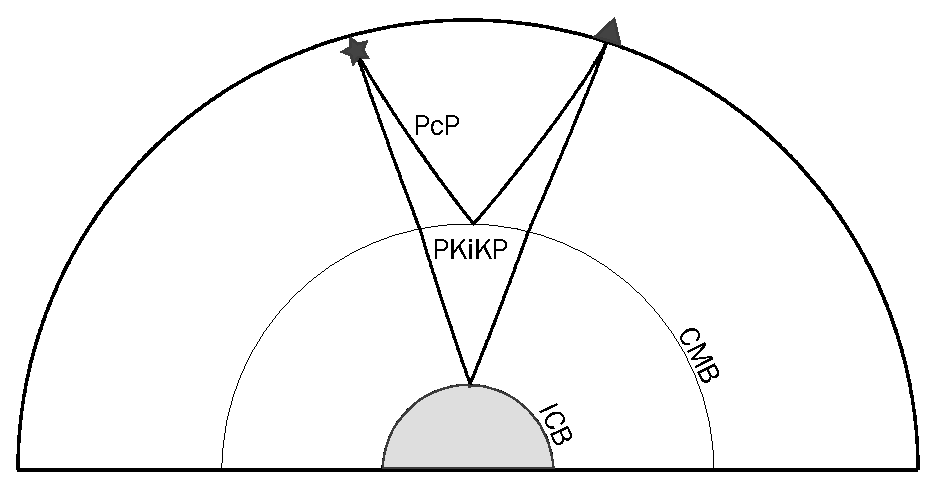
\includegraphics[width=0.7\linewidth]{fig/chap1/ray_path}
\caption{PcP和PKiKP射线路径示意图}
\label{fig:ray_path}
\end{figure}

\section{PKiKP/PcP振幅比的强烈离散}
作为内核冷凝增长和内核与外核相互作用的场所~\citep{Deguen2011,Bergman2010},地球的内外核边界(ICB)的物理性质一直也是地震学的重要问题之一. 到目前为止,对ICB的研究基本都是利用由该界面反射的PKiKP震相,而PKiKP也是内核存在最为直接的证据. PKiKP又分为前临界和后临界,在早期的观测条件下,后临界PKiKP(又被成为PKP${}_{df}$)的观测要更为容易,其作为参考震相,通常与PKP${}_{bc}$结合,被用于研究内
核顶部的结构~\citep{Tanaka1997}. 相比而言,由于较小的反射系数和较低的信噪比,加上观测条件的限制,
在早期对于小震中距情况下的前临界PKiKP的观测数量非常有限~\citep{Bolt1970},但还是有研究尝试利用PKiKP/PcP振幅比来估计内核的密度和ICB波速跃变~\citep{Souriau1989,Shearer1990}. 由于PcP和PKiKP在浅部结构中传播路径的相似性(图\ref{fig:ray_path}),这种使用振幅比的
方法假设可以消除地幔结构、台站响应等因素对观测结果的影响而且CMB是平坦且横向变化不大的,观测到振幅比异
常则来自内核,由此估计ICB的物理参数. \citet{Krasnoshchekov2005}用记录到核爆事件产生的PKiKP绝
对振幅来约束ICB的区域变化,推测出内核表面存在马赛克结构. 虽然振幅经过了震级校正,但台站的增益及场地效
应依然是不确定的因素. 因此,关于ICB的研究大多使用PcP作为参考震相. 随着近年来大规模地震台阵的安装和区
域性密集台网的布设,PKiKP的观测数量显著提升,通过搜索全球1995至2000年的IMS小口径台阵数据,利用叠加方法,\citet{Koper2004a}搜集了三百多个PKiKP观测,远远超过之前的观测数量的总和;利用Hi-net,\citet{Kawakatsu2006}首次报道了由一个地震产生的超过100个清晰的PKiKP记录,通过慢度分析和波形拟合,有
力地证实了尖锐ICB的存在. 虽然PKiKP的观测数量大大提升,但用它和PcP约束内核参数仍然面临很多困难. 首先
在小震中距情况下,PcP容易被S波的尾波干扰,因此限制了可用的数据量;其次,由于台阵口径有限,PKiKP在内核的反射有限,很难将所有采样区域的观测结果联系起来并结合地球动力学机制进行讨论~\citep{Tanaka2015a};再次,即使在很小的区域,观测到的振幅比也可能呈现出非常离散~\citep{Koper2004a},但造成数据离散
的来源却很难确定. 

大量观测表明内核并不是一个物性均一的刚性球体,除了波速的各向异性~\citep{Wang2015},现在也已有较多的
观测证据支持内核内部的不均匀性结构,像1-degree的东西半球的速度和衰减的不均匀~\citep{Tanaka1997,Wen2002}和内核顶部局部的小尺度散射结构~\citep{Vidale2000a}等. 一些地球动力学模型试图对这些结构的成因给出解释,如既有外核大尺度的非对称流~\citep{Aubert2008,Gubbins2011},也有来
自内核自身的内部对流~\citep{Alboussiere2010,Monnereau2010},但还没有一种模式能完全解释地震观
测. ICB是连接内外核的桥梁,因此可能对内核结构作出一定反映,因而一些最近的研究尝试将全球的PKiKP/PcP
振幅比和走时分布与内核的东西半球差异这种模式联系起来,但由于全球数据的离散,这种尝试看上去并不可行~\citep{Waszek2015a}. 

PKiKP/PcP振幅比和走时残差的区域性离散可能有多种来源. 其一,尽管PcP和PKiKP的离源
角相差不大,它们在的传播路径还是有一定差异,因此在地壳和地幔中的所经历的衰减和不均匀性结构也会有所不同,
从而贡献振幅比和走时差的异常~\citep{Tkalcic2010a};其二,由于PKiKP射线较PcP更陡,其受到横向结构
变化的影响较小,尤其是二者受震源附近和近台站下方的结构影响的差异;其三,也是本研究关注的主要内容,如前
面所述,CMB结构会不仅会造成PcP振幅的剧烈变化,其走时也会受到影响~\citep{Koper2003}. 然而,CMB对观
测的影响却很少被之前很多研究所提及或仅有少许讨论~\citep{Cao2004,Waszek2015a,Dai2012,Tanaka2015a}. 即使注意到了可能的CMB效应,使用之前的分析方法也很难将造成数据离散的来源确定~\citep{Koper2004a}. 除了以上因素,台站的信噪比条件同样不能忽视,因为PcP和PKiKP的到时不同,而两者被记录时的信噪比
环境也不相同. 综合上面的考虑,如果不能将每种来源小心地区分出来,用振幅比和走时残差的方法就很难得到真实
的ICB物理参数的估计. 

\section{本研究的主要工作}
由于短周期PcP(1--2Hz)对CMB结构变化敏感,能提供对该界面性质最直接的约束,且PKiKP 和PcP的振幅比呈现强烈离散,而异常可能源于CMB结构对PcP的影响,这就使得可以通过振幅比的变化推测CMB结构变化. 另外,以PKiKP作为参考震相,不仅可以减小由浅部结构产生的不确定性还可以有效判断引起PcP波形变化的来源. 因而利用PcP和PKiKP研究CMB结构变化存在很好的可行性,

本硕士论文的主要工作是首先通过收集全球IMS(International Miscellaneous Stations)小口径台阵记录到的PcP和PKiKP数据,从中筛选出产生同时被两个邻近小口径台阵记录到PKiKP和PcP信号的地震事件,这两个台阵的震中距也相近,通过对比两个台阵的观测包括PKiKP
和PcP的振幅比、走时残差和波形来确定产生区域性离散的PKiKP/PcP振幅比的来源;当没有两个相近震中距的相
邻台阵的时候,通过分析多个相邻地震产生的被同一台阵记录到的PKiKP和PcP信号,并结合前人的研究结果,来推
断观测异常的成因. 利用IMS小口径台阵,不仅可以提高观测的可靠性,得出对于某个台阵的平均振幅比,以此有效
评估台阵观测的可信度,而且经过对不同台阵、地震事件和震相的比较后,一些可能对观测造成影响的因素可以被排
除,并且确认CMB的界面起伏变化和低速结构可以基本上解释PKiKP/PcP振幅比在小尺度范围内的强烈离散以及PcP的
变化. 虽然研究使用的还是常规的走时和振幅分析方法,但通过运用以上对比方法,有效地改善了对CMB小尺度结构
的分辨能力. 除了IMS小口径台阵的观测,本研究还补充了国家测震台网的数据,利用大规模的采样来分析大尺度范围内的CMB结构变化. 为了评价单台站的观测结果和分析不确定性的来源,本研究还对重复地震的PKiKP和PcP数据进行了分析和比较. 最后,尝试将本研究的观测结果和之前的地球动力学模拟结合起来,简要讨论CMB各种变化的形成机制. 